%%% Richard James Howe 1/2
%% Final Year Project poster presentation.
% This uses a package called 'baposter.cls' which can be
% found here: http://www.brian-amberg.de/uni/poster/
% This package has been written by Brian Amberg (baposter@brian-amberg.de)

\documentclass[a1paper,portrait]{baposter}

\usepackage{relsize}    % For \smaller
\usepackage{url}      % For \url
\usepackage{epstopdf}  % Included EPS files automatically converted to PDF to include with pdflatex

%%% Global Settings %%%%%%%%%%%%%%%%%%%%%%%%%%%%%%%%%%%%%%%%%%%%%%%%%%%%%%%%%%%

\graphicspath{{pix/}}  % Root directory of the pictures 
\tracingstats=2      % Enabled LaTeX logging with conditionals

%%% Color Definitions %%%%%%%%%%%%%%%%%%%%%%%%%%%%%%%%%%%%%%%%%%%%%%%%%%%%%%%%%

\definecolor{bordercol}{RGB}{40,40,40}
\definecolor{headercol1}{RGB}{186,215,230}
\definecolor{headercol2}{RGB}{80,80,80}
\definecolor{headerfontcol}{RGB}{0,0,0}
\definecolor{boxcolor}{RGB}{186,215,230}

%%%%%%%%%%%%%%%%%%%%%%%%%%%%%%%%%%%%%%%%%%%%%%%%%%%%%%%%%%%%%%%%%%%%%%%%%%%%%%%%
%%% Utility functions %%%%%%%%%%%%%%%%%%%%%%%%%%%%%%%%%%%%%%%%%%%%%%%%%%%%%%%%%%

%%% Save space in lists. Use this after the opening of the list %%%%%%%%%%%%%%%%
\newcommand{\compresslist}{
  \setlength{\itemsep}{1pt}
  \setlength{\parskip}{0pt}
  \setlength{\parsep}{0pt}
}

%%%%%%%%%%%%%%%%%%%%%%%%%%%%%%%%%%%%%%%%%%%%%%%%%%%%%%%%%%%%%%%%%%%%%%%%%%%%%%%
%%% Document Start %%%%%%%%%%%%%%%%%%%%%%%%%%%%%%%%%%%%%%%%%%%%%%%%%%%%%%%%%%%%
%%%%%%%%%%%%%%%%%%%%%%%%%%%%%%%%%%%%%%%%%%%%%%%%%%%%%%%%%%%%%%%%%%%%%%%%%%%%%%%

\begin{document}
\typeout{Poster rendering started}

%%% Setting Background Image %%%%%%%%%%%%%%%%%%%%%%%%%%%%%%%%%%%%%%%%%%%%%%%%%%
\background{
  \begin{tikzpicture}[remember picture,overlay]%
  \draw (current page.north west)+(-2em,2em) node[anchor=north west]
  {
\includegraphics[height=1.1\textheight]{background}};
  \end{tikzpicture}
}

\begin{poster}{
  grid=false,
  borderColor=bordercol,
  headerColorOne=headercol1,
  headerColorTwo=headercol2,
  headerFontColor=headerfontcol,
  boxColorOne=boxcolor,
  headershape=roundedright,
  headerfont=\Large\sf\bf,
  textborder=rectangle,
  background=user,
  headerborder=open,
  boxshade=plain
}
{
  Eye Catcher, empty if option eyecatcher=false - unused
}
{\Large\sf\bf
  A VHDL based educational computer (1/2).
}
{
  \vspace{1em} Richard James Howe : 082060589\\
  {\smaller howe.r.j.89@gmail.com}
}
{
\setlength\fboxsep{0pt}
\setlength\fboxrule{0.5pt}
  \fbox{
    \begin{minipage}{10em}
      
\includegraphics[width=10em,height=4em]{aston.jpg}
    \end{minipage}
  }
}

\headerbox{Task}{name=task,column=0,row=0}{
\smaller
\begin{itemize}
    \item Design a working computing system.
    \begin{itemize}
        \item CPU Core.
        \item RAM.
        \item I/O Interface.
        \item UART.
    \end{itemize}
    \item Create Assembler.
    \item Make Bootloader.
    \item Make test programs.
\end{itemize}
}


\headerbox{Github}{name=github,column=0,below=task}{
\smaller

The code for this project (Makefiles, VHDL, C, Forth, etc.) are
hosted on Github and can be found here:

\url{https://github.com/howerj/fyp}

\begin{center}
    
\includegraphics[scale=0.5]{qr_howerjGit.png}
\end{center}

}

\headerbox{References}{name=references,column=0,below=github, above=bottom}{
\smaller                          % Make the whole text smaller
\vspace{-0.4em}                     % Save some space at the beginning
\bibliographystyle{plain}              % Use plain style
\renewcommand{\section}[2]{\vskip 0.05em}    % Omit "References" title
\begin{thebibliography}{1}              % Simple bibliography with widest label of 1
\itemsep=-0.01em                    % Save space between the separation
\setlength{\baselineskip}{0.4em}          % Save space with longer lines
\bibitem{j1core} James Bowman, Willow Garage: \emph{J1: A small Forth CPU for FPGAs},  EuroForth 2010, \url{http://www.excamera.com/files/j1.pdf} (2010)
\bibitem{vgacore} Javier Valcarce: \emph{VHDL Macro: VGA80x40}, VHDL Monochrome VGA display adapter ,\url{http://www.javiervalcarce.eu/wiki/VHDL_Macro:_VGA80x40} (2009)
\bibitem{uartcore} Peter Bennett: \emph{RS232 UART (VHDL)}, A UART core, \url{http://bytebash.com/2011/10/rs232-uart-vhdl/} (2012)
\bibitem{opencore} Opencores: \emph{Open source HDL cores and code}, \url{http://opencores.org/projects} (2013)
\bibitem{nexysDigilent} $Nexys^{TM}$3: \emph{A FPGA Spartan-6 development board}, \url{http://www.digilentinc.com/Products/Detail.cfm?NavPath=2,400,897\&Prod=NEXYS3}, (2013)
\end{thebibliography}
} 

\headerbox{VHDL}{name=vhdl,span=2,column=1,row=0}{
\smaller
\subsection{The Project}

\begin{center}
    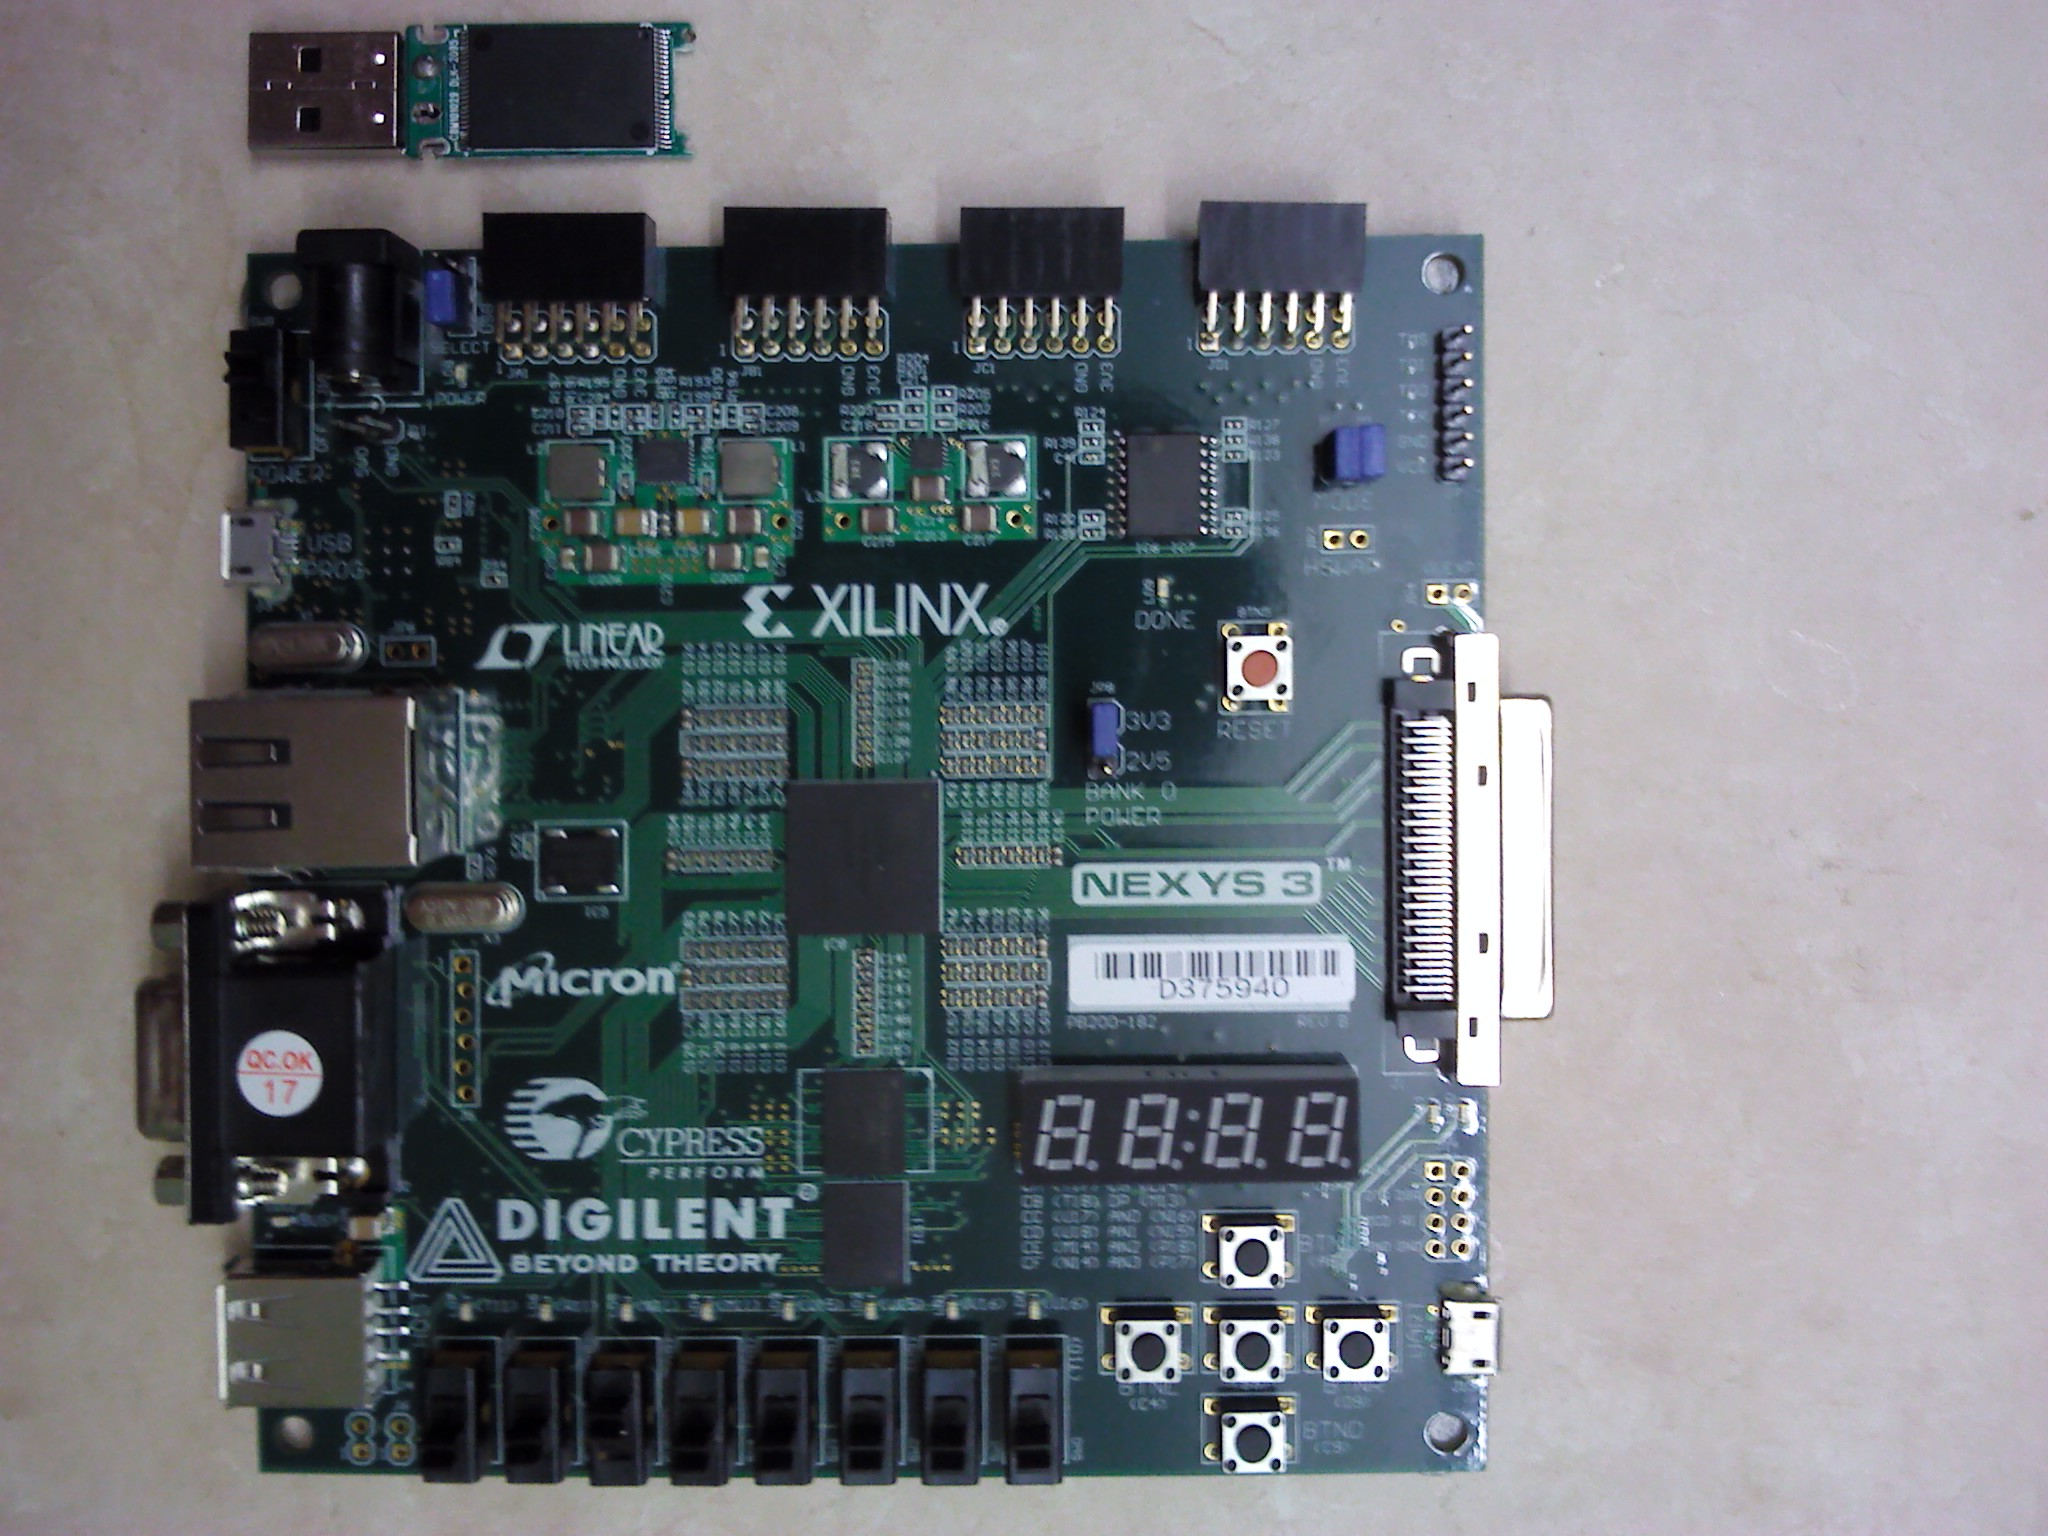
\includegraphics[scale=0.1]{devBoard.jpg}
\end{center}

Using a Nexys 3 Development board\cite{nexysDigilent}, as shown above,
I have created a portable computing system in VHDL intended for students
like myself. The project is extensible and modular, and as I have said
it is also portable using no resources specific to Xilinx, this would
allow the system to be moved to smaller, cheaper devices.

The CPU core is based around a processor originally written in Verilog
called the J1\cite{j1core}. This has been rewritten in VHDL, modified
and improved on to include new instructions and allow for greater
flexibility . The processor is stack based which allows for a system which uses
less space and can execute many FORTH instructions natively.

\subsection{Resource Utilization}
The entire system takes up very little room on the device (6slx16csg324-3)
on the development board. This would allow for further expansion of
the system and even multiple processor cores running simultaneously. Alternatively
it could mean porting to a cheaper system while not reducing any functionality.
\begin{center}
    \begin{itemize}
        \item Slice Registers : 295 out of 18224 (1\%).
        \item Slice LUTs: 789 out of 9112 (8\%).
        \item BRAMs 
            \begin{itemize}
                \item 4096x8 bit dual-port RAM, 2 (VGA Memory).
                \item 8192x16 bit dual-port RAM, 1 (CPU Core).
            \end{itemize}
    \end{itemize}
\end{center}

In addition to these, also not listed is adders, comparators, multiplexers, etcetera,
that have also been used by the design.
}

\headerbox{Firmware}
{name=firmware,span=2,column=1,below=vhdl,above=bottom}{
\smaller

The firmware is a simple bootloader, instead of compiling the program in, as you would
once the development is over, I have made a simple program that resides on the device
that allows you to load an arbitrary program onto the core. 

In order to both help me out with the build (converting file formats) and to fill the
role of an assembler and decided to go with a language I had written (FORTH) that is particularly
well suited to the task, the assembler requires just a few hundred more lines of code
to define what is necessary and the original language can be called from it.

% Made with my own Forth interpreter.
% Bootloader.
}

\end{poster}
\end{document}
